\chapter{System architecture}
\label{sec:architecture}
\thispagestyle{fancy}

To satisfy the requirements specified in the previous section a system can be designed in terms of a number of data structures used to store the index and statistics data and a number of major components. For data the data structures it is chosen to implement three types of indices - content index, occurrence index, and document statistics index. The major components of the system are chosen to be a buffer manager to handle disk I/O, a feeder chosen to feed the text files into the system, an indexer chosen to construct and store index, a query retrieval part chosen to process textual queries using the stored index, score the candidate results and generate {\it snippets} for the top-scored results, a clustering component that may perform result clustering and cluster scoring based on provided snippets, and finally a front end part chosen to be a dedicated web-server. In addition the system has to contain a number of components for performance evaluation, unit testing and debugging.

\section{Index Structures}
The system is designed around three major data structures, or indices. These are the occurrence index which stores inverted lists with positions. The content index stores the content of the documents, and is used for snippets and clustering. The last index is the statistics index which is used to store document statistics which may be used to calculate relevance. 

\subsection{Document and statistics index structure}\label{sub:statistics_index_structure}
The statistics index is a mapping from document id to a statistics object containing information such as most frequent term, document vector $tf*idf$ length and number of unique terms.

\subsection{Content index structure}\label{sub:content_index_structure}
The content index stores the content of the documents indexed, these documents are stored as lists of raw document tokens, with nothing being added or removed. By concatenating any consecutive subsequence of tokens a section of the original document can be produced. The last property is used when extracting snippets.  

\subsection{Occurrence index structure}\label{sub:occurrence_index_structure}
The occurrence index consists of two parts, a dictionary and an inverted file. The dictionary contains the indexed terms, and a pointer into the inverted file. The inverted file contains an inverted list for each term stored in alphabetical order. The inverted list of a term contains all the documents occurrences of this term sorted by increasing document ID. Each document occurrence contains a list the positions within the document where the term occurs. The index structure is shown in Figure~\ref{fig:occ_index_struct}.

\begin{figure}[h!!tb]
	\centering
	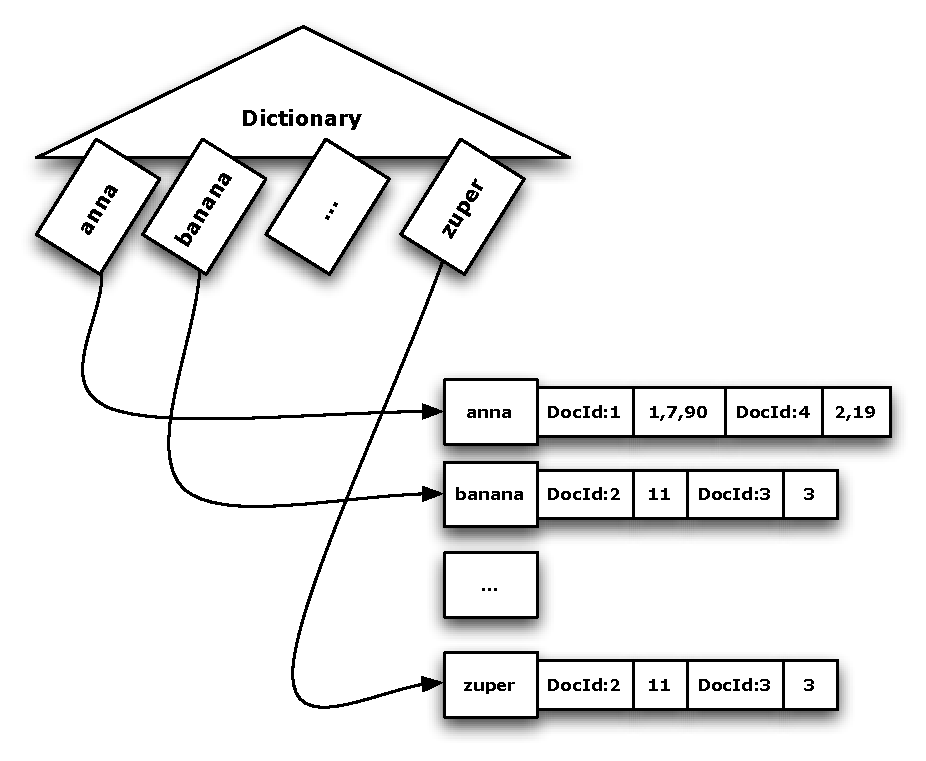
\includegraphics[width=0.8\textwidth]{include/index.pdf}
	\caption[Occurrence index structure]{Occurrence index structure.}\label{fig:occ_index_struct}
\end{figure}

\section{Buffered IO}\label{sec:buffered_io}
To solve one of the major bottlenecks of search, namely disk I/O a buffer manager can be used. A buffer manager can split files into blocks and, when a part of a file is requested for reading or writing, it may fetch it entirely from disk into a memory buffer, eventually saving time on later requests to the same file area. However, the memory used by a buffer manager is limited to a certain number of buffers and a buffer size; newly fetched buffers has to replace already stored buffers. The easiest way to handle buffers replacement is to use a Least Recently Used (LRU) replacement policy. In addition, the buffer manager has to implement flushing of dirty buffers, but the technicalities of the buffer manager implementation are quite irrelevant for the context of this assignment and, if needed, they can be obtained from the source code itself.

\section{Feeding pipeline}\label{sec:feeding_pipeline}
An important processing stage during the document indexing is feeding of the data into the indexer. The approach of transforming of the input data into a stream of document terms is chosen to use a {\it feeding pipeline}. The pipeline proposed as a solution is based on two main concepts. Frist, the structure chosen to represent a document is an object containing various objects with various keys (fields), which is basically a map. Second, a pipeline processor can transform a field in a document structure, and place the result in an other processor. 

An example of a feeding processor is illustrated by Figure~\ref{fig:feeding_processor}. Finally, the output of the feeding pipeline is submitted to the indexer process described in next section. 

\begin{figure}[htb]
	\centering
	
\includegraphics[width=0.9\textwidth]{include/processor.pdf}
	\caption[Feeding pipeline example]{Feeding pipeline example, a html to text processor strips away html from the input field ``content'', and puts the result into the ``cleaned'' field.}\label{fig:feeding_processor}
\end{figure}

\subsection{Feeding processors}\label{sub:implemented_feeding_processors}
To be able to solve the task the feeding pipeline has to implement multiple feeding processors. These are:

\begin{itemize}
	\item \textbf{HtmlToText:} strips away HTML tags.
	\item \textbf{Tokenizer:} breaks the documents into tokens. These tokens are raw document tokens with no characters removed from the text, the text is only split into pieces.
	\item \textbf{PunctuationRemover:} removes punctuation and whitespace characters from tokens. 
	\item \textbf{Stemmer:} reduces tokens to their stems. 
	\item \textbf{Termizer:} creates inverted documents, collecting position lists for each term in the document.
\end{itemize}

\section{Index building}\label{sub:index_building}
When building the indices, all the documents fed into the system are given a unique document ID from a global counter.

The occurrence index is built in two phases: in the first phase documents are converted to inverted lists and combined into one inverted list representing one index update. When the index is flushed, the index update that was built in the first phase is merged with the existing inverted index. Since the inverted lists are sorted on term, document and position merging the lists is a trivial task. However, during this merge, the statistics for each document have to be re-calculated and stored in the statistics index. Finally, when the merge is completed, the dictionary is updated so that the pointers in the dictionary point into the newly created inverted file.

\section{Query processing}
The query processing part of the system is designed to be both flexible and extensible. The main idea is to have a query processor which uses a query preprocessor and a number of query processing components to produce and sort query results. A query preprocessor uses a number of built-in stages (similar to those used for the document processing) to transform a textual query into a query structure.

A query processing component, on the other hand, is an abstract component that may be used to pull query results. Each component may include another component as a source, and it is possible to construct a chain of such components. To begin with, a minimal number of processing components has to include:
\begin{itemize}
	\item {\bf Matcher:} produces a number of combined results for a given query. These match inclusion and exclusion of terms based on AND, OR and NAND modifiers.
	\item {\bf Score Combiner:} pulls results from its source and scores them according to a number of score modules that can be added to the system. The system may implement a number of different similarity models (both dynamic and static) and a score combiner can calculate a weighted average from these.
	\item {\bf Filters:} may filter out some of the results based on a number of abstract filters that can be later implemented and added to the system.
\end{itemize}

\begin{figure}[ht]
	\centering
	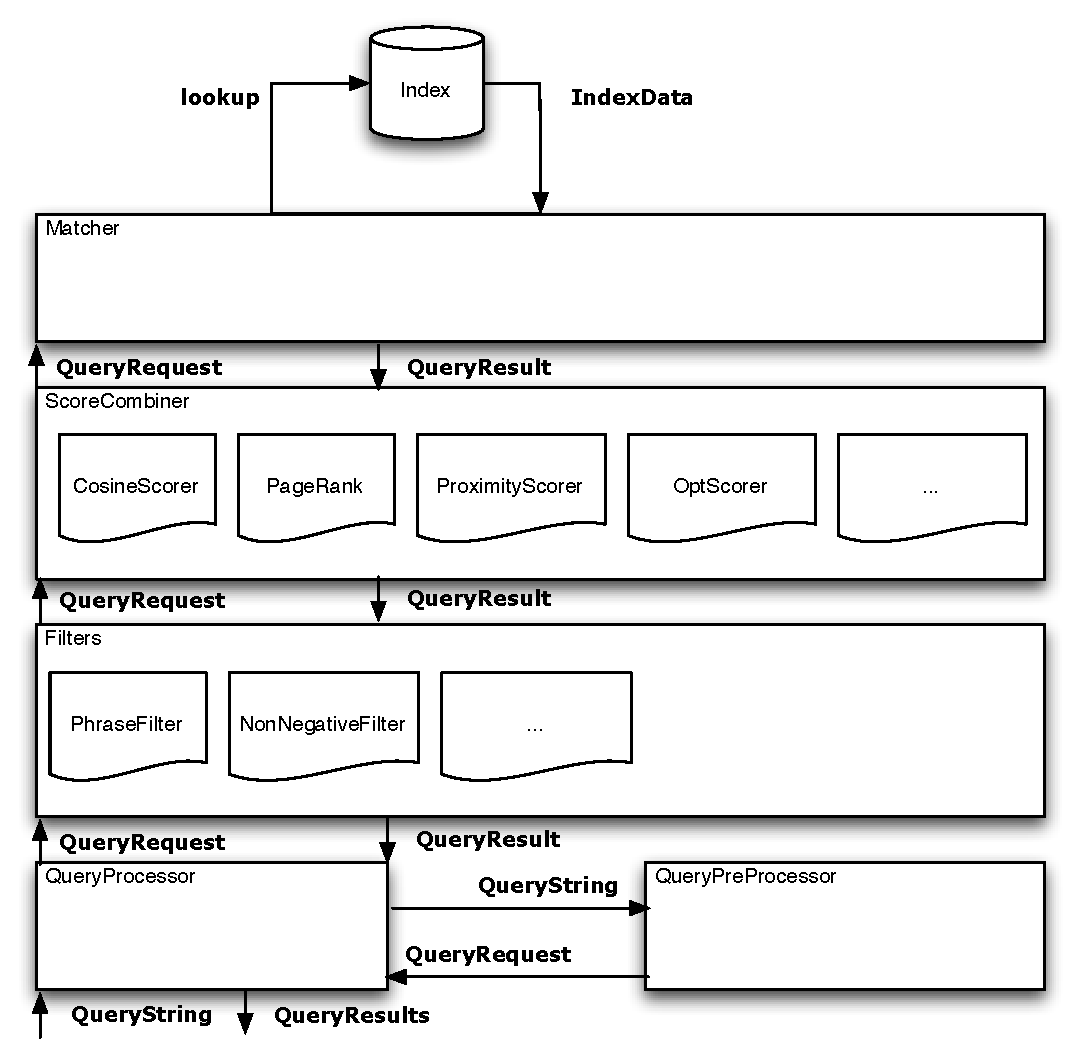
\includegraphics[width=0.9\textwidth]{include/query_processing.pdf}
	\caption{Query processing subsystem.}\label{fig:query_processing}
\end{figure}

The most important point here is that the query processor does not have to know what components are used in the query processing, and a system implementation is free to extend the number of components, add several instances of the same component in the processing pipeline or change the processing order of these. 

In future, the system may be extended by a merger that enables to merge a number of processing pipelines into one. In this case, the system may become distributed. For example, it may run a number of basic matchers, scorers and filters on a number of different nodes, then results from these may be pulled together by a new merger component which may combine the results. If required, the processing pipeline may be extended by a couple of new filters and scorers used to re-weight and filter the combined results. However, due to the project duration limits the target search engine is chosen to run only on a single computer.

The query processing structure proposed for an initial implementation of Solbrille is illustrated by Figure~\ref{fig:query_processing}. The rest of this section explains the basic processing components and the ideas behind.

\subsection{Matcher component}
The matcher component is the part of the processing pipeline which performs the actual lookups in the inverted index. The matcher extracts the various terms referenced in a query and executes one lookup for each term. It also recognizes the modifiers associated with the terms (\emph{AND}, \emph{OR} and \emph{NAND}). The matchers purpose is to create candidate results for further filtering and ranking. A candidate result is a document which satisfies the query. That is, a document where \emph{all} terms with a \emph{AND} modifier is present and \emph{no} terms with a \emph{NAND} modifier. In addition the terms with \emph{OR} modifiers are appended to the documents which satisfies the \emph{AND} and \emph{NAND} requirements.

The matcher component allows to support a limited subset of boolean queries, however, since it has no aspect of parenthesises the subset is rather small. For vector space queries, all terms are treated with \emph{OR} modifiers.

\subsubsection{Critique and an alternative approach (A Postnote)}\label{sssub:matcher_critique}
To support the full range of boolean queries a tree of \emph{AND}, \emph{OR} and \emph{NAND} matching components could be constructed. This would be a much more flexible way of building result candidates. Merging all functionality for doing matching into one component also leads to one piece of very complex code.

The reason a more general scheme was not used were that an index term could have been looked up multiple times. However, this is not a issue with the proposed design of the buffer manager and processing component. Since the results are pulled one by one and combined as soon as possible, a repeated request to the same term will be cached in the buffer manager. Therefore the performance impact of this general scheme is close to nothing. 

\subsection{Score Combiner and Scorer Components}
The idea with score combiner is to retrieve a number of score values from different scorers, and then combine these into a total score. The main intention here is that the system may implement different scoring models or even combine these. A scorer may implement a cosine model, a probabilistic model such as Okapi BM-25, a static link-analysis models such as PageRank or HITS, or even an Opt model\footnote{the optimal model with 1.0 in both precision and recall, an inside joke}.

To be fast, some of the document collection statistics later required by scorers have to be stored in the query requests and query results, since the access to global statistics on demand may be too slow. 

\subsection{Filters and Phrase Search}
To demonstrate the idea with filters the system is intended to present two types of filters, a non-negative filter and a phrase filter. A non-negative filter is rather a demonstation of the concept and it can just filter out the results which have a score value less or equal to zero. However, using the scorer components specified above, this situation is impossible.

A phrase filter has a more practical application. The main intention is to filter results based on + and - phrases.

A simple case for the phrase search is either a phrase such as {\it +''kari bremnes''} or a phrase like {\it kari +''kari bremnes''}. The solution for both of these is to represent AND phrases as lists of terms in the query structure, match and score the corresponding terms just as normal terms, and then finally check if these terms occur in the required order using the document occurrence part of the inverted index.

A more problematic case for the phrase search is a query such as {\it kari -''kari bremnes''}. In this case the user wants to retrieve all the documents containing word {\it kari}, but not the word {\it kari} followed by the word {\it bremnes}.

The solution is to introduce a fourth modifier type, PNAND. As for the AND phrases, the query structure has to store a number of phrases represented as a modifier (AND or NAND) and a list of terms. All the terms represented in a phrase has the same modifier as the phrase itself, and terms having both PNAND and an other modifier have to loose the PNAND modifier. The matcher component has to perform a match on both NAND, OR and AND terms, and also PNAND terms interpreted as OR terms. Any scorer component has then to ignore PNAND terms, giving 0 in the score impact of these. Any results matching either NAND phrases of only PNAND terms have to be removed in the phrase filter.

Finally, in the current design a result says to be filtered out if one of the filters does not approve the result. This approach can be later extended to use a boolean expression of filter constraints, represented as a tree or similar.

\subsubsection{Critique and an Alternative Approach (A Postnote)}
The approach described above was chosen to be implemented, just to demonstrate the idea behind the filtering component. However, as the phrase filtering is now performed during all the stages of the query processing pipeline this method is rather impractical. A better solution that can be applied in future is to use a separate phrase matcher, and then combine the matched phrase results and the ordinary term results before sending these to a scorer component. The same alternative solution as the one mentioned in Section~\ref{sssub:matcher_critique} with respect to multiple index lookups applies here as well.

\subsection{Final Details for Result Scoring}
To save memory the results pulled by the query processor are stored into a priority queue. As a query is expected to be a query string and a page range {\it startpage} end {\it endpage}, the maximum queue size is limited by {\it endpage}. When the queue size has reached this value a new candidate has to be compared with the least scored result contained in the queue. If the candidates value is greatest of these two, the candidate has to replace the least scored result in the priority queue.

When all the results are processed, up-to {\it endpage} - {\it startpage} results has to be extracted from the queue, sorted in descending order and returned to the user.

\subsection{Snippet extraction}\label{sub:snippet_extraction}
To ensure a pleasant user experience, search results should contain a short piece of the original document. This snippet could be the beginning of the document, however, since the occurrence index contains the positions of the various terms it should be possible to select more suitable snippets. 

The simple scheme selected for the snippet extraction is that the position lists for all the terms in the query are merged to one list. Then a {\it snippet window} which contains the greatest number of queries terms. The length of the window is a predefined constant, and the unit of the window dimensions is number of terms.

\subsubsection{Critique and an Alternative Approach (A Postnote)}
Selecting the window with the highest number of matching tokens is not a good measure of snippet relevance. Common words and stop-words will be counted as much as any other word. Treating the various possible snippet-windows as documents and calculating their relevancy to the query could be a better solution, however, efficient algorithms to do this have not been studied. 

To produce visual appealing search result presentations the length of the snippet windows could have been calculated in number of characters rather than number of tokens. Using tokens as the unit of measure the variance of the snippet lengths might be high. 

\section{Extended System}

For the extended system,  a clustering technique that is based on suffix trees is used. The methods is presented in \cite{zamir} which have been used as a reference when developing the clustering technique.

\subsubsection{Suffix Tree} 

A suffix tree is a representation of a text which speeds up several string algorithms. In a suffix tree, all suffixes of a text is held in  a trie to speed up string comparisons, meaning that algorithms like substring comparison can be done in $O(m)$ time (where $m$ is the size of the substring). In a naive implementation of a suffix tree, creation time and space would be $O(n^2)$, but when using an algorithm called Ukkonen's algorithm, both time and space can constraints can be reduced to $O(n)$. More information can be found in \cite{suffixtreebook}.

Usually in a suffix tree, charcters is chosen as the most atomic part of a text. For this project words was chosen as the most atomic part. The primary reason for this is that substring matches is not of interset, since term frequency is used to score matches. To support using words as atomic parts, and to support having multiple documents in a tree, a variant of suffix trees called Generalized Suffix Tree is used . This is a tree that resembles a normal suffix tree, but which also has a bit set on each node, which describes which documents contain that node. 

\subsubsection{Suffix Tree Clustering}

The clustering method itself is based on the method as presented in \cite{zamir}. What is basically done is that for every document in the result set, the snippet is extracted and put into the suffix tree. For all terms and phrases that excists in more than one document, the tree will then contain a node where the cardinality of the bit set is more than 1. A simple iteration over the tree will then extract all common phrases and terms. This is again used to create clusters of documents, where all the documents have a set of phrases in common.

Since there are usually a lot of "garbage" nodes (common words, words/phrases that only occur in one document, or nodes which contains every result in the result set), every node is scored. The score function depends on the number of words in phrase, if the words are common or not, the score calculated by the scorer and the number of documents that share the phrase. 

The N best nodes is then chosen and joined. All nodes where more than half of each set are in both sets are then joined. For the joined sets,  all nodes where the phrases are simple subsets of eachother is removed. For example, if "president kennedy" and "kennedy" containes the same documents, "kennedy" is removed, to leave the most expressive of the two.

Finally, all the clusters (joined nodes) are rescored, and all clusters which has a score that wis more than 1/5th of the maximum cluster score.

\section{Front-End Design}
The main responsibilities to the front-end is to handle and provide search functionality to a user. This can be done through embedding Jetty in the system. Jetty is a compact java web server which supports both embedded and stand-alone deployment of applications. Embedding Jetty gives us advantages such as reducing the complexity of the development environment, requires no installation, and in-line configuration of the web server. However, it increases the complexity of writing views because of the in-line configuration.

Jetty is configured and started by a front-end component. The idea is to have two context paths, where a context path is a domain where a given set of services are accessible. The two different context paths are used for servlets and serving of static content such as documents and images. The currently proposed servlets are:

\begin{itemize}
\item {\tt A search servlet}: This is the main servlet that handles the search functionality of the application.
\item {\tt A feeder servlet}: A hook for feeding the search application with documents.
\end{itemize}

The current system proposal embeds mark-up generation in the servlets. This is a huge disadvantage as the code complexity of each servlet increases drastically. A future improvement would be to introduce the Model-View-Controller architectural pattern, and separate the servlet and the markup. Another improvement would be to not embedding jetty, and create a generic web application which is able to run using any java web server. However, this would require a installation of the chosen web server.

\section{Testing}
Test-driven development is proposed to be used to ensure the quality of the most important components. During development, the tests can be designed and made before each component is implemented. A test is composed of one or several test cases, and in order to pass, all conditions must be correct. {\bf JUnit} is used for implementing test cases, and they will be located in a separate web-tree.

\subsection{A Postnote}
The current test coverage is rather limited. Currently, only the {\it feeder}, {\it index}, {\it buffering} and {\it system} components are covered by tests. This is due to the fact that test development takes time, and were substituted by manual testing at the end of this project when time became limited. In future, the test coverage can be improved.